% vim: ft=tex spell spelllang=en ts=2 sw=2 et

\setchaptertoc
\chapter{Implementation}

This chapter provides both guidance to browse the \Eol* source
code~\cite{eol-github}, and insight into the details worth
mentioning of the implementation of the system.

% \enlargethispage{2\baselineskip}
\afterintro


\section{Project Source Structure}

The \Eol* source code is organized in the following directory structure, which
follows usual conventions for C projects:

\begin{figure}[h]
    \centering
    \noindent\begin{minipage}{0.75\textwidth}
\dirtree{%
.1 \DtFolder{lua-eol/}.
.2   \DtFolder{doc/} \DTcomment{Documentation and API reference}.
.2   \DtFolder{examples/}.
.3     *.lua \DTcomment{Module usage examples}.
.2   \DtFolder{tools/} \DTcomment{Build \& test utilities}.
.3     \DtFolder{ninja/} \DTcomment{Ninja build support files}.
.3     \DtFolder{make/} \DTcomment{GNU Make build support files}.
.2   \DtFolder{test/}.
.3     *.lua \DTcomment{Unit tests}.
.2   uthash.h \DTcomment{Copy of UT-hash}.
.2   eol-*.c \DTcomment{Module sources}.
.2   eol-*.h \DTcomment{Module sources}.
}
    \end{minipage}
    \caption{Source tree structure.}
\end{figure}

Module source files (\verb|eol-*.h|, \verb|eol-*.c|) are named after the
components identified during the design phase. In particular:

\begin{itemize}

  \item \verb|eol-module.c| \hfill\\
    Main part of the code, including the interfacing with Lua.

  \item \verb|eol-fcall.h|,
        \verb|eol-fcall-<name>.h|,
        \verb|eol-fcall-<name>.c|... \hfill\\
    Different implementations of the native function invocation mechanism.

  \item \verb|eol-typing.h|, \verb|eol-typing.c| \hfill\\
    Type representation module.

  \item \verb|eol-typecache.h|, \verb|eol-typecache.c|, \verb|uthash.h| \hfill\\
    Type representation cache module.

  \item \verb|eol-libdwarf.h|, \verb|eol-libdwarf.c| \hfill\\
    Utility functions to simplify working with \verb|libdwarf|.

  \item \verb|eol-lua.h| \hfill\\
    Utility functions to simplify working with the Lua C API.

  \item \verb|eol-trace.h|, \verb|eol-trace.c| \hfill\\
    Tracing support module.

  \item \verb|eol-util.h|, \verb|eol-util.c| \hfill\\
    Miscellaneous utility code, including support code for the runtime checks.

\end{itemize}


\section{Type Representation}

Converting values from C to Lua, and vice versa, is one of the most important
tasks performed by \Eol*: C values need to be made accessible from Lua.
Therefore, this information needs to be read from the DWARF debugging
information (see \nameref{sec:debuginfo-structure}), and kept around in
a suitable data structure. This structure must be:

\begin{itemize}
  \item Exhaustive, to hold all the needed information.
  \item Compact, to minimize memory usage.
\end{itemize}

Describing base types is possible using just an enumerated type: there is
a fixed amount of them, and the characteristics (size, name, etc) are well
known. The challenging part is representing user defined types (\Mc|struct|,
\Mc|enum|, \Mc|union|), and derived types (pointers, arrays).

The data structure for describing types is \verb|EolTypeInfo|
(\autoref{lst:EolTypeInfo}). It is a tagged \Mc|struct|, with the tag
indicatingthe type kind (\verb|EOL_TYPE_S32| for 32-bit signed integers,
\verb|EOL_TYPE_STRUCT| for a \Mc|struct|, etc; the complete list of values
can be seen in \autoref{lst:EolType}). The contained data will vary
depending on the value of the \emph{kind} tag. The members for all possible
values are grouped in an \Mc|union| in order to make them share the
same memory space.

\begin{listing}[H]
  \begin{ccode}
    struct _EolTypeInfo {
      EolType type;
      union {
        struct TI_base     ti_base;
        struct TI_pointer  ti_pointer;
        struct TI_typedef  ti_typedef;
        struct TI_const    ti_const;
        struct TI_array    ti_array;
        struct TI_compound ti_compound;
      };
    };
    typedef struct _EolTypeInfo EolTypeInfo;
  \end{ccode}
  \caption{\texttt{EolTypeInfo}.}
  \label{lst:EolTypeInfo}
\end{listing}

\begin{listing}[tH]
  \centering
  \begin{ccode}
    typedef enum {
      EOL_TYPE_VOID,    /* void        */
      EOL_TYPE_BOOL,    /* _Bool       */
      EOL_TYPE_S8,      /* int8_t      */
      EOL_TYPE_U8,      /* uint8_t     */
      EOL_TYPE_S16,     /* int16_t     */
      EOL_TYPE_U16,     /* uint16_t    */
      EOL_TYPE_S32,     /* int32_t     */
      EOL_TYPE_U32,     /* uint32_t    */
      EOL_TYPE_S64,     /* int64_t     */
      EOL_TYPE_U64,     /* uint64_t    */
      EOL_TYPE_FLOAT,   /* float       */
      EOL_TYPE_DOUBLE,  /* double      */
      EOL_TYPE_TYPEDEF, /* typedef … T */
      EOL_TYPE_CONST,   /* const T     */
      EOL_TYPE_POINTER, /* T*          */
      EOL_TYPE_ARRAY,   /* T …[n]      */
      EOL_TYPE_STRUCT,  /* struct …    */
      EOL_TYPE_UNION,   /* union …     */
      EOL_TYPE_ENUM,    /* enum …      */
    } EolType;
  \end{ccode}
  \caption{\texttt{EolType} enumeration.}
  \label{lst:EolType}
\end{listing}


\begin{table}[f]
  \centering
  \begin{tabular}{lll}
    \toprule
    C Construct     & DWARF DIE                    & \Eol* Type            \\
    \midrule
    \Mc|void|       & ø                            & \Mc|EOL_TYPE_VOID|    \\
    \Mc|bool|       & \verb|DW_TAG_base_type|      & \Mc|EOL_TYPE_BOOL|    \\
    \Mc|int8_t|     & \verb|DW_TAG_base_type|      & \Mc|EOL_TYPE_S8|      \\
    \Mc|uint8_t|    & \verb|DW_TAG_base_type|      & \Mc|EOL_TYPE_U8|      \\
    \Mc|int16_t|    & \verb|DW_TAG_base_type|      & \Mc|EOL_TYPE_S16|     \\
    \Mc|uint16_t|   & \verb|DW_TAG_base_type|      & \Mc|EOL_TYPE_U16|     \\
    \Mc|int32_t|    & \verb|DW_TAG_base_type|      & \Mc|EOL_TYPE_S32|     \\
    \Mc|uint32_t|   & \verb|DW_TAG_base_type|      & \Mc|EOL_TYPE_U32|     \\
    \Mc|int64_t|    & \verb|DW_TAG_base_type|      & \Mc|EOL_TYPE_S64|     \\
    \Mc|uint64_t|   & \verb|DW_TAG_base_type|      & \Mc|EOL_TYPE_U64|     \\
    \Mc|float|      & \verb|DW_TAG_base_type|      & \Mc|EOL_TYPE_FLOAT|   \\
    \Mc|double|     & \verb|DW_TAG_base_type|      & \Mc|EOL_TYPE_DOUBLE|  \\
    \Mc|typedef|... & \verb|DW_TAG_typedef|        & \Mc|EOL_TYPE_TYPEDEF| \\
    \Mc|const|...   & \verb|DW_TAG_const_type|     & \Mc|EOL_TYPE_CONST|   \\
    ...\Mc|*|       & \verb|DW_TAG_pointer_type|   & \Mc|EOL_TYPE_POINTER| \\
    ...\Mc|[n]|     & \verb|DW_TAG_array_type|     & \Mc|EOL_TYPE_ARRAY|   \\
    \Mc|struct|...  & \verb|DW_TAG_structure_type| & \Mc|EOL_TYPE_STRUCT|  \\
    \Mc|union|...   & \verb|DW_TAG_union_type|     & \Mc|EOL_TYPE_UNION|   \\
    \Mc|enum|...    & \verb|DW_TAG_enumration_type|& \Mc|EOL_TYPE_ENUM|    \\
    \bottomrule
  \end{tabular}
  \caption{Mapping of C types, DWARF DIEs and \Mc|EolType|.}
\end{table}

\noindent
The following sections describe in detail the members of \verb|EolTypeInfo|.


\subsection{Base Type Representation}

\begin{ccode*}{samepage=true}
  struct TI_base {
    char               *name;
    uint32_t            size;
  };
\end{ccode*}

\noindent
Even though it is sufficient to provide type kind codes for all the base types
as discussed before, providing the possibility of querying their \verb|name|
and \verb|size| is a convenient feature, at a very small cost: the
\verb|EolTypeInfo| value for each one of the base types is a singleton,
defined as follows:

\begin{ccode*}{samepage=true}
  /* File: eol-typing.h */
  extern const EolTypeInfo* eol_typeinfo_u32;

  /* File: eol-typing.c */
  const EolTypeInfo* eol_typeinfo_u32 = &((EolTypeInfo) {
    .kind         = EOL_TYPE_U32,
    .ti_base.name = "uint32_t",
    .ti_base.size = sizeof (uint32_t),
  });
\end{ccode*}

\noindent In practice, to avoid writing the definitions of all the base types,
the C preprocessor and a couple generator macros are used (see
\autoref{sec:cpp-abuse-genmacros}).


\subsection{Pointer Representation}
  \label{sec:pointer-typeinfo}

\begin{ccode*}{samepage=true}
  struct TI_pointer {
    const EolTypeInfo *typeinfo;
  };
\end{ccode*}

\noindent
Pointers are represented by referencing the \verb|EolTypeInfo| of the
pointed-to type. Thus, it is the only member in \Mc|struct TI_pointer|. The
size of a pointer value is platform dependent, but well known and constant for
each platform, and is the value of the C expression \Mc|sizeof(void*)|.


\subsection{Array Representation}

\begin{ccode*}{samepage=true}
  struct TI_array {
    const EolTypeInfo *typeinfo;
    uint64_t           n_items;
  };
\end{ccode*}

\noindent
Arrays are represented by referencing the \verb|EolTypeInfo| of the array
items, plus the number of items (\verb|n_items|) present in the array. The
size of an array value can be calculated multiplying the size of the item type
by the number of items in the array.


\subsection{User Defined Type Representation}

\begin{ccode*}{samepage=true}
  struct TI_compound {
    char             *name;
    uint32_t          size;
    uint32_t          n_members;
    EolTypeInfoMember members[];
  };
\end{ccode*}

\noindent This record type represents all user defined types: enumerated types
(\Mc:enum:), record types (\Mc:struct:), and union types (\Mc:union:):

\begin{description}
  \item [\Mc|name|] \hfill \\
    User defined types are usually given a name, but it is optional and in
    this case the value will be \Mc|NULL|.
  \item [\Mc|size|] \hfill \\
    Contains the size of the type, in bytes.
  \item [\Mc|n_members| / \Mc|members|] \hfill \\
    Count of members (or enumerators, for \verb|EOL_TYPE_ENUM|) in the type,
    and an array contaning their descriptions. Using
    a \gls{flexible-array-member}, allows usage of a single chunk of memory
    for the \verb|EolTypeInfo| itself and the items in the array.
\end{description}

\noindent
The auxiliar \verb|EolTypeInfoMember| type is defined as follows:

\begin{ccode*}{samepage=true}
  typedef struct {
    const char            *name;
    union {
      int64_t              value; /* enum */
      struct {                    /* union, struct */
        uint32_t           offset;
        const EolTypeInfo *typeinfo;
      };
    };
  } EolTypeInfoMember;
\end{ccode*}

\noindent
This always contains the (optional) \Mc|name| of the types, and usage of the
remaining fields varies with the type being described:

\begin{itemize}
  \item For \Mc|EOL_TYPE_STRUCT|, the \Mc|offset| of the member (in bytes,
    from the beginning of the record) and a pointer to its type information
    (\Mc|typeinfo|) are used.
  \item For \Mc|EOL_TYPE_UNION|, the \Mc|offset| is ignored, and only the
    type information of the member (\Mc|typeinfo|) is used.
  \item For \Mc|EOL_TYPE_ENUM|, only the \Mc|value| associated with the
    enumerator is used.
\end{itemize}

\noindent
An \Mc|union| is used to make fields share the same memory space.


\subsection{Type Alias Representation}

\begin{ccode*}{samepage=true}
  struct TI_typedef {
    char              *name;
    const EolTypeInfo *typeinfo;
  };
\end{ccode*}

Type aliases assign a name to an arbitrary type. They are represented by the
\Mc|name| and a pointer to the \Mc|EolTypeInfo| of the type.


\subsection{Read-only Type Representation}

\begin{ccode*}{samepage=true}
  struct TI_const {
    const EolTypeInfo *typeinfo;
  };
\end{ccode*}

\noindent
Flagging a type as read-only (i.e. using the \Mc|const| type qualifier in C)
is represented in the same way as pointers (\autoref{sec:pointer-typeinfo}):
by keeping a pointer to the \Mc|EolTypeInfo| that is read-only.




\section{Type cache}
  \label{sec:impl-type-cache}

The type cache is implemented as an opaque data structure which can only be
used by means of its public API (\autoref{lst:eol-typecache-api}). Internally
it is implemented as a hash table which reuses uthash~\cite{uthash-guide}, and
it maps integer keys (\Mc|uint32_t|) to \Mc|EolTypeInfo| structures. Cache
keys can be any integer which uniquely identifies a particular type.
For a \Mc|EolTypeInfo| created from its DWARF representation, the offset of
the top-level \gls{DIE} is used as the key. This works because information for
a particular type is never duplicated inside the same ELF file, so there is an
unique offset in the file for it.

\begin{listing}[tH]
  \centering
\begin{ccode}
typedef struct _EolTypeCacheEntry* EolTypeCache;

typedef bool (*EolTypeCacheIter)  (EolTypeCache*,
                                   const EolTypeInfo*,
                                   void *userdata);

void eol_type_cache_init (EolTypeCache *cache);
void eol_type_cache_free (EolTypeCache *cache);

void eol_type_cache_add (EolTypeCache      *cache,
                         uint32_t           offset,
                         const EolTypeInfo *typeinfo);

const EolTypeInfo* eol_type_cache_lookup (EolTypeCache *cache,
                                          uint32_t      offset);

void eol_type_cache_foreach (EolTypeCache    *cache,
                             EolTypeCacheIter callback,
                             void             *userdata);
\end{ccode}
  \caption{Public API of \Mc|EolTypeCache|}.
  \label{lst:eol-typecache-api}
\end{listing}

The type cache only manages its own dynamically allocated memory, used for the
nodes of the hash table. The \Mc|EolTypeInfo| structures referenced by the
cache are considered opaque by the cache, and the memory used by them is not
ever freed by the cache: freeing the cache leaks memory if the cached entries
are not freed by other means. In practice, this is not a problem because the
type information is constructed as-needed, and cached during the whole
lifetime of each loaded ELF object. This approach allows to simply iterate
over the elements to free each one of them before unloading the object file.


\section{Memory Ownership and Life Cycle}

Native code uses a different approach for memory management compared to Lua:
while Lua uses \gls{GC}, which handles freeing chunks of memory automatically,
native code frees memory explicitly. Take for example a function which creates
a new \Mc|struct| and returns it:

\begin{ccode*}{samepage=true}
struct point { int x; int y; };

struct point* point_new (int x, int y) {
  struct point *p = malloc (sizeof (struct point));
  p->x = x;
  p->y = y;
  return p;
}
\end{ccode*}

Then, that code is built into an ELF shared object file (\verb|point.so|),
which is loaded using \Eol*, and used normally:

\begin{luacode}
local Geometry = eol.load("point.so")
local point = Geometry.point_new(1, -1)
-- Use the point normally.
\end{luacode}

The Lua VM only knows the userdata that \Eol* has created to represent the
returned value, but it is not aware of the memory that has been allocated to
hold the \Mc|struct point| value. Once the value is not used anymore by the
Lua program, the garbage collector reclaims the space used by the userdata,
but \verb|free()| is not called to free the memory allocated by
\verb|malloc()|. Lua just does not know about memory that it has not allocated
itself. One solution is to manually call a function to free the memory from
Lua:

\begin{luacode}
local libc = eol.load("libc.so")
libc.free(point)
point = nil  -- Make sure it won't be used
\end{luacode}

The main problem with this is that the automatic memory management done by the
Lua VM is lost, and programmers are forced to write additional code to free
memory regions. This puts a burden in the developer, which would rather be
avoided.


\subsection{Lua as a Custom Allocator}
  \label{sec:userdata-lua-custom-allocator}

The Lua VM exposes in its C API the ability to create \emph{userdata} objects.
For the VM, userdata is seen as an opaque value which, by default, cannot be
manipulated from Lua; for the client code using the Lua API, an userdata value
is a region of memory allocated by the Lua VM, which can contain any data.
Like every other value managed by the VM, userdata is subject to \gls{GC},
which means that userdata values which are no longer referenced by a Lua
program are garbage collected. This effectively allows C programmers to reuse
the Lua GC for their data.

\begin{listing}[tH]
  \centering
  \begin{ccode}
  struct data { /* ... */ };

  void initialize_data (struct data *d);

  struct data* push_new_data (lua_State *L) {
    struct data *d = lua_newuserdata (L, sizeof (struct data));
    initialize_data (d);
    return d;
  }
  \end{ccode}
  \caption{Using Lua userdata to store values}
  \label{lst:values-in-userdata}
\end{listing}

By default, userdata values have no predefined behaviour in Lua, except for
assignment (which also covers passing userdata values as function parameters),
and testing for identity. Assigning a metatable to an userdata value allows
the programmer to define operations on userdata values.


\subsubsection{GC Finalization}

The only thing known by the Lua VM about userdata values is that they are
a region of memory. That means that Lua will only free the memory region when
the userdata is picked by the \gls{GC}. If the userdata contains resources
other than raw memory (a file handle, for example), it must be ensured that
those are released appropriately. In order to coordinate the GC with the
management of resources unknown to the VM, Lua supports defining
\emph{finalizer} functions.

Lua requires the programmer to explicitly mark userdata to be finalized. This
is done by setting its metatable: if the metatable contains a function (the
finalizer) associated to the \Mlua|__gc| key, it is called after the userdata
is marked by the GC as garbage, with the userdata itself being passed as the
only argument. Once the userdata is finalized, the memory used by it will be
normally released by Lua. The finalizer can be a C function, allowing native
code to release any resources used by userdata.

Using finalizers is needed when dealing with opaque types which are handled
via pointers. The standard C library includes such a type: open files in C are
handled using pointers to \Mc|FILE| values (for an example, see
\autoref{lst:c-fileptr}), which are created when opening a file with
\Mc|fopen()|. Files cannot be deallocated directly, and instead the
\Mc|fclose()| function must be used. \autoref{lst:lua-gc-example-module}
contains a complete example of a Lua module implemented in C which uses a
finalizer to ensure that opened files are properly closed calling
\Mc|fclose()| from the finalizer.

\begin{listing}[tH]
    \begin{ccode}
    int main (int argc, char **argv) {
        FILE *fd = fopen ("hello.txt", "w");
        fprintf (fd, "Hello, C file!\n");
        fclose (fd);
        return 0;
    }
    \end{ccode}
    \caption{Using an opaque \Mc|FILE*| in C.}
    \label{lst:c-fileptr}
\end{listing}

Finalizers are used extensively in the implementation of the \Eol* Lua module.
The module's own userdata types need finalization (details on those are
provided in \autoref{sec:eol-mod-typemeta}), and it also allows to attach
arbitrary Lua functions to values created by native code wrapped in an
\Mc|EolVariable| userdata.


\begin{listing}[tH]
  \small
  \begin{center}
    \emph{C code, to be built with \texttt{cc -shared -o openlog.so
    openlog.c}}
  \end{center}
\begin{ccode}
struct logger {
  FILE *output;
};

static int logger_call (lua_State *L) { /* ... */ }

static int logger_gc (lua_State *L) {
  struct logger *l = luaL_checkudata (L, 1, "LOGGER");
  if (l->output) fclose (l->output); /* Close the file */
  return 0;
}

static int logger_new (lua_State *L) {
  const char *path = luaL_checkstring (L, 1);
  lua_Integer verbosity = luaL_checkinteger (L, 2);
  struct logger *l = lua_newuserdata (L, sizeof (struct logger));
  if (!(l->output = fopen (path, "a")))
    return luaL_error (L, "cannot open (\%s)", strerror (errno));
  l->verbosity = (int) verbosity;
  luaL_setmetatable (L, "LOGGER");
  return 1;
}

int luaopen_openlog (lua_State *L) {
  static const luaL_Reg metamethods[] = {
    { "__call", logger_call, }
    { "__gc", logger_gc, }
    { NULL, NULL },
  };
  luaL_newmetatable (L, "LOGGER");
  luaL_setfuncs (L, metamethods, 0);
  lua_pushcfunction (L, logger_new);
  return 1;
}
\end{ccode}

  \begin{center}
    \emph{Using the module from Lua}
  \end{center}

\begin{luacode}
  local openlog = require("openlog")
  local log = openlog("/var/log/example.log", true)
  log("Log line")
\end{luacode}

  \caption{Small C module which demonstrates using a \texttt{\_\_gc} metamethod}
  \label{lst:lua-gc-example-module}
\end{listing}


\section{\Eol* Lua module}

The top-level API exposed to Lua is the \verb|eol| module, which has to be
returned by the C function that the Lua VM calls after loading an extension
module. This function is always called \verb|luaopen_<module>|, where
\verb|<module>| is the name of the module being loaded:

\begin{ccode}
LUAMOD_API int
luaopen_eol (lua_State *L)
{
  eol_trace_setup ();

  (void) elf_version (EV_NONE);
  if (elf_version (EV_CURRENT) == EV_NONE)
    return luaL_error (L, "outdated libelf version");

  luaL_newlib (L, eollib);
  create_meta (L);
  return 1;
}
\end{ccode}

Notice how the function uses \verb|luaL_newlib()| instead of manually creating
a table in the Lua stack, and setting a field for each one of the \verb|eol.*|
module level functions. The \verb|eollib| variable is defined as follows,
using the supplied \verb|luaL_Reg| type:

\begin{ccode}
static const luaL_Reg eollib[] = {
  { "load",     eol_load     },
  { "type",     eol_type     },
  { "sizeof",   eol_sizeof   },
  { "typeof",   eol_typeof   },
  { "offsetof", eol_offsetof },
  { "cast",     eol_cast     },
  { NULL, NULL },
};
\end{ccode}

As a last step, \verb|create_meta()| is called to register the metatables for
the C types which \Eol* exposes to the Lua VM (\vref{sec:eol-mod-typemeta}).


\subsection{Userdata Metatables}
  \label{sec:eol-mod-typemeta}

Metatables for the userdata types (\textsf{Library}, \textsf{Function},
\textsf{CType}, and \textsf{Variable}) are created when the \Eol*
module is loaded by the Lua VM, in the \verb|create_meta()| C function.
Exactly one metatable for each type is created, and all the userdata values of the same
type share the same metatable. All metatables have some common entries:

\begin{itemize}

  \item A \verb|__gc| metamethod, responsible for decreasing the reference
  count of the associated \textsf{Library}.

  \item A \verb|__tostring| metamethod, in order to provide a string
  representation of the values of the userdata. This is used by the Lua
  \Mlua|tostring()| function.

  \item A \verb|__index| metamethod, which provides support for indexing the
  userdata. The concrete behavior depends on the type of the userdata.

\end{itemize}

For each metatable, an array of \Mc|struct luaL_Reg| values is created. It
contains a list of metamethods and pointers to the C functions which implement
them. The example below is for \textsf{Library}; the rest share a strong
similarity:

\begin{ccode}
/* Methods for Library userdata. */
static const luaL_Reg library_methods[] = {
    { "__gc",       library_gc       },
    { "__tostring", library_tostring },
    { "__index",    library_index    },
    { "__eq",       library_eq       },
    { NULL, NULL }
};
\end{ccode}

Then, in the \verb|create_meta()| function, the metatable is created with the
aid of the \verb|luaL_newmetatable()| utility function, which arranges for the
metatable to be available for checking the types of a userdata value later on
with the companion functions \verb|luaL_checkudata()| and
\verb|luaL_testudata()|:

\begin{ccode}
static void
create_meta (lua_State *L) {
    /* EolLibrary */
    luaL_newmetatable (L, EOL_LIBRARY);
    luaL_setfuncs (L, library_methods, 0);
    lua_pop (L, 1);

    /* ... */
}
\end{ccode}

\todo[inline]{Got time? Describe how lookups are done, it is relatively interesting}

\subsection{Library loading}

The implementation of \verb|eol.load()| tries to avoid loading the same
library more than once. If a library is loaded, its reference count is
incremented, and the returned \textsf{Library} userdata contains a reference
to the previously loaded library. To achieve this behavior while preserving
reference bookkeeping simple, a linked list of loaded libraries is maintained.
Each \verb|EolLibrary| \Mc|struct| contains a pointer to the \verb|next|
library (which can be \Mc|NULL|):

\begin{ccode}
struct EolLibrary {
  /* Members used for bookkeeping */
  unsigned int       ref_counter;
  const char        *path;
  struct EolLibrary *next;

  /* Other members */
  /* ... */
};
\end{ccode}

The \verb|path| of libraries is used to determine if two libraries are the
same. For this to work, the \verb|path| of a library, and the paths of
libraries which are candidates to be loaded must must be in canonical form
as returned by the \verb|realpath()|\footnote{\texttt{realpath()}
canonicalizes a file path, it is part of the POSIX standard and included in
most Unix-like systems.} function before comparing them.

It would have been possible to use a hash table to map library paths
(canonicalized) to their corresponding \verb|EolLibrary| \Mc|struct|, to
determine in constant time whether a library is loaded, instead of the linear
time required to check a linked list. However, most programs use, on average,
a number of libraries in the order of tens, and reading the DWARF sections
which contain the index of available types and symbols is much more costly for
any non trivial library. Therefore, it was determined that the linked list
solution would suffice, while avoiding the additional complexity of the hash
table.


\subsection{Type Information Lookup}

Looking up type information is one of the most common operations performed by
\Eol*. As per the design (\autoref{sec:design-overview}), type information is
to be stored in the \textsf{Type Cache} (for details of its implementation,
see \autoref{sec:impl-type-cache}). It seemed convenient to provide a single
entry point for all the type information lookups which always checks the
\textsf{Type Cache}. This function is \verb|library_lookup_type()|:

\begin{ccode}
static const EolTypeInfo*
library_lookup_type (EolLibrary  *library,
                     Dwarf_Off    d_offset,
                     Dwarf_Error *d_error) {
    const EolTypeInfo *typeinfo =
            eol_type_cache_lookup (&library->type_cache, d_offset);
    if (!typeinfo) {
        typeinfo = library_build_typeinfo (library, d_offset, d_error);
        eol_type_cache_add (&library->type_cache, d_offset, typeinfo);
    }
    return typeinfo;
}
\end{ccode}

It is important to note that the cache is always checked first: on a cache
hit, the cached values are returned immediately, while in the event of a cache
miss a call to the \verb|library_build_typeinfo()| is used to create a new
\verb|EolTypeInfo| from the DWARF debugging information, which is always added
to the cache \emph{right away}. This is especially important because
\verb|EolTypeInfo| values can contain references to others, which in turn
cause additional type information lookups. Having the intermediate values
built also added in the cache greatly increases the ratio of cache hits. To
better understand this, consider the following example lookups for functions
of the C standard library, starting from an empty cache:

\begin{figure}[thH]
  \centering
  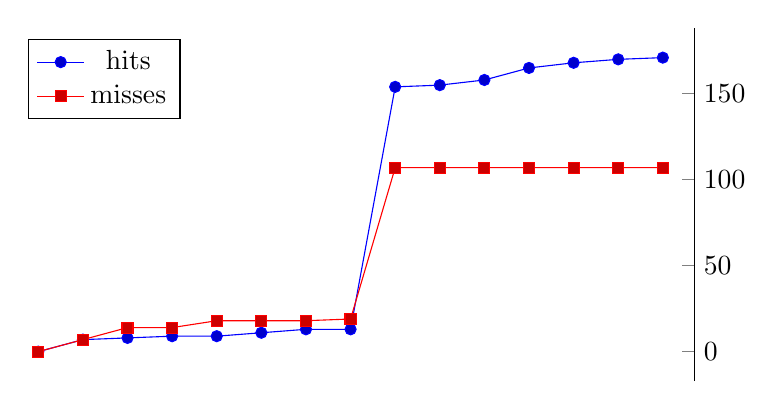
\begin{tikzpicture}
    \begin{axis}[
      width=0.85\textwidth,
      height=0.5\textwidth,
      style={/pgf/number format/assume math mode=true},
      % xlabel={\emph{time$\rightarrow$}},
      % ylabel={\emph{hits / misses}},
      enlarge x limits=0.05,
      axis on top,
      tick align=inside,
      axis x line=none,
      axis y line*=right,
      legend style={legend pos=north west},
      x tick label style={opacity=0},
    ]
      \addplot plot coordinates {
        (1,0) (2,7) (3,8) (4,9) (5,9) (6,11) (7,13) (8,13) (9,154) (10,155)
        (11,158) (12,165) (13,168) (14,170) (15,171)
      };
      \addplot plot coordinates {
        (1,0) (2,7) (3,14) (4,14) (5,18) (6,18) (7,18) (8,19) (9,107)
        (10,107) (11,107) (12,107) (13,107) (14,107) (15,107)
      };
      \legend{hits \\ misses \\}
    \end{axis}
  \end{tikzpicture}
  \caption{Typical progression of type cache hits/misses over time}
  \label{fig:plot-type-cache-hitmiss}
\end{figure}

\begin{enumerate}

  \item Lookup type information for the \Mc|int atoi(const char*)| function.
  This generates one lookup for the \Mc|int| return type, plus another lookup
  for the \Mc|const char*| parameter. The latter causes itself more lookups:
  one for the \Mc|char*| type, which itself causes yet another lookup for the
  \Mc|char| type. The type information for \Mc|char| gets added to the
  cache at this point, then the information for \Mc|char*|, and finally for
  \Mc|const char*|.

  \item Lookup type information for the \Mc|char* strchr(const char*, int)|
  function. The cache already contains the type information for the function
  parameters, which were looked up for the \Mc|atoi()| function. The type
  information for the return type, \Mc|char*|, is already in the cache,
  because it has been added as a partial result for the \Mc|atoi()|
  function. As for the parameter types, \Mc|const char*| is also
  in the cache.

\end{enumerate}

The implemented policy for type information lookup quickly fills up the cache
as fast as possible while the program starts, up to a point where most of the
types used are all present in the cache
(\autoref{fig:plot-type-cache-hitmiss}), and from that moment onwards the
amount of cache misses is very small. 


\subsection{Querying Types}

The \verb|eol.typeof()| function accepts arguments of different types.
The \verb|luaL_check*()| family of functions from the Lua C API raise an error
if the argument does is not of the expected type, and therefore some
additional work is needed to ensure that it works as specified:

\begin{ccode}
static int
eol_typeof (lua_State *L) {
  if (luaL_testudata (L, 1, EOL_TYPEINFO)) {
    lua_settop (L, 1);
  } else {
    EolVariable *ev = luaL_testudata (L, 1, EOL_VARIABLE);
    if (ev) {
      typeinfo_push_userdata (L, ev->typeinfo);
    } else {
      luaL_checktype (L, 1, LUA_TSTRING);
      const char *name = lua_tostring (L, 1);
      /* Omitted: Lookup type by name in all loaded libraries */
      typeinfo_push_userdata (L, typeinfo);
    }
  }
  return 1;
}
\end{ccode}

Functions \verb|eol.sizeof()|, \verb|eol.alignof()|, and \verb|eol.offsetof()|
are implemented similarly, with the exception that they omit the code to
look up the type information when passing a string argument. Once the
corresponding \verb|EolTypeInfo| is found, it can be queried for the requested
information: \verb|eol_typeinfo_sizeof()| to obtain the size,
\verb|eol_typeinfo_alignment()| for the alignment, and for obtaining the
offset of a \Mc|struct| member, the information is available in the
\verb|EolTypeInfoMember| value returned by the
\verb|eol_typeinfo_compound_named_member()|.

\subsection{Casting}

Using the \verb|eol.cast()| function on a \textsf{Variable} userdata changes
the associated type for it, effectively treating the same data as if it were
of another type. In order to achieve this, we just return to Lua a new
\textsf{Variable} userdata with the given type information which points to
the same memory area:

\begin{ccode}
static int
eol_cast (lua_State *L) {
  const EolTypeInfo *typeinfo = to_eol_typeinfo (L, 1);
  EolVariable *ev = to_eol_variable (L, 2);

  /* Use typeinfo from 2nd argument, same data address. */
  variable_push_userdata (L, ev->library, typeinfo,
    ev->address, ev->name, VARIABLE_NOCOPY);
  return 1;
}
\end{ccode}


\subsection{Preprocessor “Generator Macros”}
  \label{sec:cpp-abuse-genmacros}

This is a programming pattern used thorough the code of \Eol*: the
C preprocessor is used in a convoluted way as a rudimentary code generator
using lists of related elements. First, a macro of related elements is defined
(\emph{enumerator macro}, from now on), and it must accept the identifier for
another macro (the \emph{generator macro}) as a parameter. Each element in the
enumerator macro is an expansion of the generator, passing the parameters
needed by the generator.

In order to better understand how generator macros work, let us walk through
a complete example adapted from the \Eol* source code. The following macro
expands into a function which checks the type of an \Mc|EolTypeInfo| — it is
the \emph{generator}:

\begin{ccode*}{samepage=true}
#define MAKE_TYPEINFO_IS_TYPE(suffix, name, ctype)            \
    bool eol_typeinfo_is_ ## name (const EolTypeInfo *înfo) \
    { return info->type == EOL_TYPE_ ## suffix; }
\end{ccode*}

\noindent In generator macros like this, the concatenation operator
(\verb|##|) of the preprocessor is used extensively to build pieces of valid
C code. The example shows how the \verb|name| parameter is concatenated to
create the name of the generated function, and the \verb|suffix| parameter is
concatenated to create a valid \verb|EolType| (\autoref{lst:EolType})
value. A valid expansion of the above macro is:

\begin{ccode*}{samepage=true}
MAKE_TYPEINFO_IS_TYPE (S32, s32, int32_t)
\end{ccode*}

\noindent
which generates the following valid C function:

\begin{ccode*}{samepage=true}
  bool eol_typeinfo_is_s32 (const EolTypeInfo *info)
  { return info->type == EOL_TYPE_S32; }
\end{ccode*}

\noindent The \emph{enumerator macro} is made by grouping a set of macro
expansions like the one above. The key is using a generic name for the
generator macro, which will be passed as a parameter. The next listing defines
an enumerator which expands a generator \verb|F| for each signed integer type:

\begin{ccode*}{samepage=true}
#define INTEGER_S_TYPES(F) \
    F (S8,  s8,  int8_t  ) \
    F (S16, s16, int16_t ) \
    F (S32, s32, int32_t ) \
    F (S64, s64, int64_t )
\end{ccode*}

\noindent Using the above definition, an expansion of the \emph{enumerator
macro} causes multiple expansions at once of the \emph{generator macro} passed
as \verb|F|, which in turn creates as many functions as elements in the
enumerator macro. In this example, using generator macros reduces the amount
of code that the programmer must write manually close to one fourth of the
original.

Another use case for generator macros is creating the code for cases in
a \Mc|switch| statement. Instead of constructing the code for an entire
function at a time, only a single \Mc|case| label and its associated
statements are generated. This is done in the following example:

\begin{ccode*}{samepage=true}
#define MAKE_SIGNED_TYPE_CASE(suffix, name, ctype) \
    case EOL_TYPE_ ## suffix: return true;

bool eol_type_is_signed (EolType type) {
  switch (type) {
    INTEGER_S_TYPES (MAKE_SIGNED_TYPE_CASE)
    default: return false;
  }
}
\end{ccode*}


\beforeintro
